\documentclass[10pt]{article}\usepackage[margin=.7in]{geometry}\usepackage{graphicx}\begin{document}\section*{Independent target-rank review}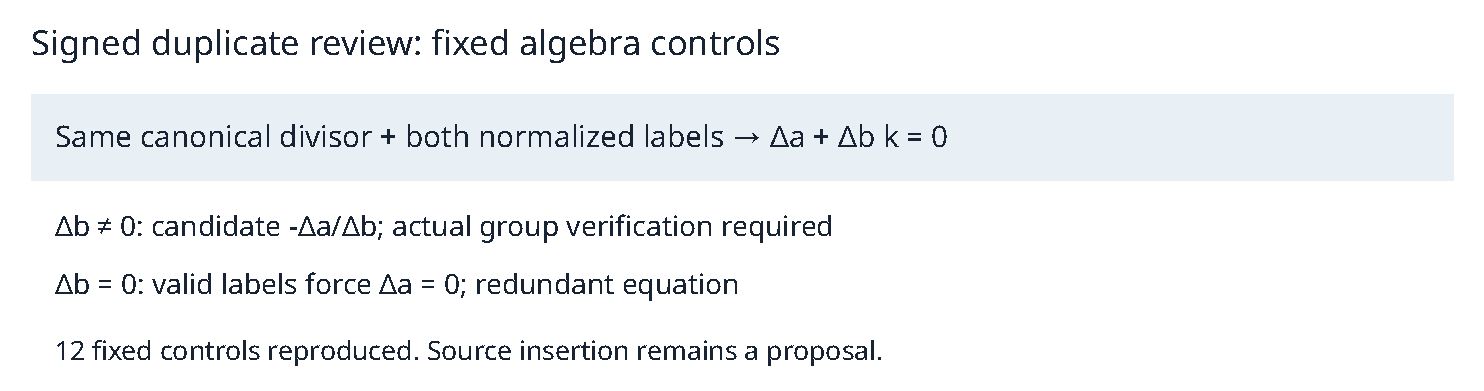
\includegraphics[width=\linewidth]{figure.pdf}
No blocking discrepancy was found in the stated algebra or proposed source placement. All producer hashes matched. One fixed-checker replay returned exit zero and reproduced the producer result byte for byte.

\paragraph{Rank controls} Forest, balanced target-bearing triangle, balanced redundant triangle and unbalanced triangle have left-nullities 0, 1, 1, 0 over F11. The balanced dependence is $(-1,-1,1)$; its target coefficient distinguishes useful and redundant equations. The graph model still requires a justified field-coordinate interpretation.

\paragraph{Source placement} The existing signed-divisor set rejects duplicates before graph insertion at pruned.rs:521. A proposed map can compare the first stored pair with the new sign-normalized pair before rejection. Both labels must receive the sign; first-occurrence graph signs and labels must remain mutually consistent. This is not implemented collector evidence.

\paragraph{Coverage} Four duplicate cases, four invalid-assumption fixtures and four rank cases were checked. The fixed F11 checker is not a generic prime-order or group validator. No naturally generated duplicate, Jacobian verification, source trajectory or historical 114-edge forest was rerun. A planted relabeling would test an interface only.

\paragraph{Artifacts} REVIEW.md provides derivations and precise limitations. status.json and receipt.json bind the replay; the manifest supplies full artifact hashes. No scientific execution or repository edit occurred.
\end{document}